\documentclass[10pt]{article}\usepackage[]{graphicx}\usepackage[]{color}
%% maxwidth is the original width if it is less than linewidth
%% otherwise use linewidth (to make sure the graphics do not exceed the margin)
\makeatletter
\def\maxwidth{ %
  \ifdim\Gin@nat@width>\linewidth
    \linewidth
  \else
    \Gin@nat@width
  \fi
}
\makeatother

\definecolor{fgcolor}{rgb}{0.345, 0.345, 0.345}
\newcommand{\hlnum}[1]{\textcolor[rgb]{0.686,0.059,0.569}{#1}}%
\newcommand{\hlstr}[1]{\textcolor[rgb]{0.192,0.494,0.8}{#1}}%
\newcommand{\hlcom}[1]{\textcolor[rgb]{0.678,0.584,0.686}{\textit{#1}}}%
\newcommand{\hlopt}[1]{\textcolor[rgb]{0,0,0}{#1}}%
\newcommand{\hlstd}[1]{\textcolor[rgb]{0.345,0.345,0.345}{#1}}%
\newcommand{\hlkwa}[1]{\textcolor[rgb]{0.161,0.373,0.58}{\textbf{#1}}}%
\newcommand{\hlkwb}[1]{\textcolor[rgb]{0.69,0.353,0.396}{#1}}%
\newcommand{\hlkwc}[1]{\textcolor[rgb]{0.333,0.667,0.333}{#1}}%
\newcommand{\hlkwd}[1]{\textcolor[rgb]{0.737,0.353,0.396}{\textbf{#1}}}%
\let\hlipl\hlkwb

\usepackage{framed}
\makeatletter
\newenvironment{kframe}{%
 \def\at@end@of@kframe{}%
 \ifinner\ifhmode%
  \def\at@end@of@kframe{\end{minipage}}%
  \begin{minipage}{\columnwidth}%
 \fi\fi%
 \def\FrameCommand##1{\hskip\@totalleftmargin \hskip-\fboxsep
 \colorbox{shadecolor}{##1}\hskip-\fboxsep
     % There is no \\@totalrightmargin, so:
     \hskip-\linewidth \hskip-\@totalleftmargin \hskip\columnwidth}%
 \MakeFramed {\advance\hsize-\width
   \@totalleftmargin\z@ \linewidth\hsize
   \@setminipage}}%
 {\par\unskip\endMakeFramed%
 \at@end@of@kframe}
\makeatother

\definecolor{shadecolor}{rgb}{.97, .97, .97}
\definecolor{messagecolor}{rgb}{0, 0, 0}
\definecolor{warningcolor}{rgb}{1, 0, 1}
\definecolor{errorcolor}{rgb}{1, 0, 0}
\newenvironment{knitrout}{}{} % an empty environment to be redefined in TeX

\usepackage{alltt}

\usepackage{amsmath,amssymb,amsthm}
\usepackage{fancyhdr,url,hyperref}
\usepackage{graphicx,xspace}
\usepackage{subfigure}
\usepackage{tikz}
\usetikzlibrary{arrows,decorations.pathmorphing,backgrounds,positioning,fit,through}

\oddsidemargin 0in  %0.5in
\topmargin     0in
\leftmargin    0in
\rightmargin   0in
\textheight    9in
\textwidth     6in %6in
%\headheight    0in
%\headsep       0in
%\footskip      0.5in

\newtheorem{thm}{Theorem}
\newtheorem{cor}[thm]{Corollary}
\newtheorem{obs}{Observation}
\newtheorem{lemma}{Lemma}
\newtheorem{claim}{Claim}
\newtheorem{definition}{Definition}
\newtheorem{question}{Question}
\newtheorem{answer}{Answer}
\newtheorem{problem}{Problem}
\newtheorem{solution}{Solution}
\newtheorem{conjecture}{Conjecture}

\pagestyle{fancy}

\lhead{\textsc{Prof. McNamara}}
\chead{\textsc{SDS/MTH 220: Lecture notes}}
\lfoot{}
\cfoot{}
%\cfoot{\thepage}
\rfoot{}
\renewcommand{\headrulewidth}{0.2pt}
\renewcommand{\footrulewidth}{0.0pt}

\newcommand{\ans}{\vspace{0.25in}}
\newcommand{\R}{{\sf R}\xspace}
\newcommand{\cmd}[1]{\texttt{#1}}
\newcommand{\Ex}{\mathbb{E}}

\rhead{\textsc{September 25, 2017}}
\IfFileExists{upquote.sty}{\usepackage{upquote}}{}
\begin{document}

\paragraph{Agenda}
\begin{enumerate}
  \itemsep0em
  \item Categorical explanatory variable
  \item Leverage, influence, and outliers
\end{enumerate}



\paragraph{Warmup: Regression}
In 1966 \href{http://en.wikipedia.org/wiki/Cyril_Burt}{Cyril Burt} published a paper called ``The genetic determination of differences in intelligence: A study of monozygotic twins reared apart." The data consist of IQ scores for [an assumed random sample of] 27 identical twins, one raised by foster parents, the other by the biological parents. 

Here is the regression output for using $Biological$ IQ to predict $Foster$ IQ:

\begin{knitrout}\footnotesize
\definecolor{shadecolor}{rgb}{0.969, 0.969, 0.969}\color{fgcolor}\begin{kframe}
\begin{alltt}
\hlkwd{library}\hlstd{(mosaic)}
\hlkwd{library}\hlstd{(faraway)}
\hlstd{m1} \hlkwb{<-} \hlkwd{lm}\hlstd{(Foster} \hlopt{~} \hlstd{Biological,} \hlkwc{data} \hlstd{= twins)}
\hlkwd{coef}\hlstd{(m1)}
\end{alltt}
\begin{verbatim}
## (Intercept)  Biological 
##    9.207599    0.901436
\end{verbatim}
\begin{alltt}
\hlkwd{rsquared}\hlstd{(m1)}
\end{alltt}
\begin{verbatim}
## [1] 0.7779022
\end{verbatim}
\end{kframe}
\end{knitrout}

\begin{enumerate}
\item Which of the following is \textbf{FALSE}? Justify your answers.

\begin{enumerate}
  \itemsep0.7in
\item Alice and Beth were raised by their biological parents. If Beth's IQ is 10 points higher than Alice's, then we would expect that her foster twin Bernice's IQ is 9 points higher than the IQ of Alice's foster twin Ashley. 
\item Roughly 78\% of the foster twins' IQs can be accurately predicted by the model.
\item The linear model is $\widehat{Foster} = 9.2 + 0.9 \times Biological$.
\item Foster twins with IQs higher than average are expected to have biological twins with higher than average IQs as well.
  \vspace{0.5in}
\end{enumerate}

\item Interpret the coefficients of the model. 
\end{enumerate}




\clearpage
\paragraph{Height and weight} The scatterplot and least squares summary below show the relationship between weight measured in kilograms and height measured in centimeters of 507 physically active individuals.
\begin{knitrout}\footnotesize
\definecolor{shadecolor}{rgb}{0.969, 0.969, 0.969}\color{fgcolor}\begin{kframe}
\begin{alltt}
\hlkwd{library}\hlstd{(openintro)}
\hlkwd{qplot}\hlstd{(}\hlkwc{data} \hlstd{= bdims,} \hlkwc{x} \hlstd{= hgt,} \hlkwc{y} \hlstd{= wgt,} \hlkwc{xlab} \hlstd{=} \hlstr{"Height (cm)"}\hlstd{,} \hlkwc{ylab} \hlstd{=} \hlstr{"Weight (kg)"}\hlstd{)}
\end{alltt}
\end{kframe}
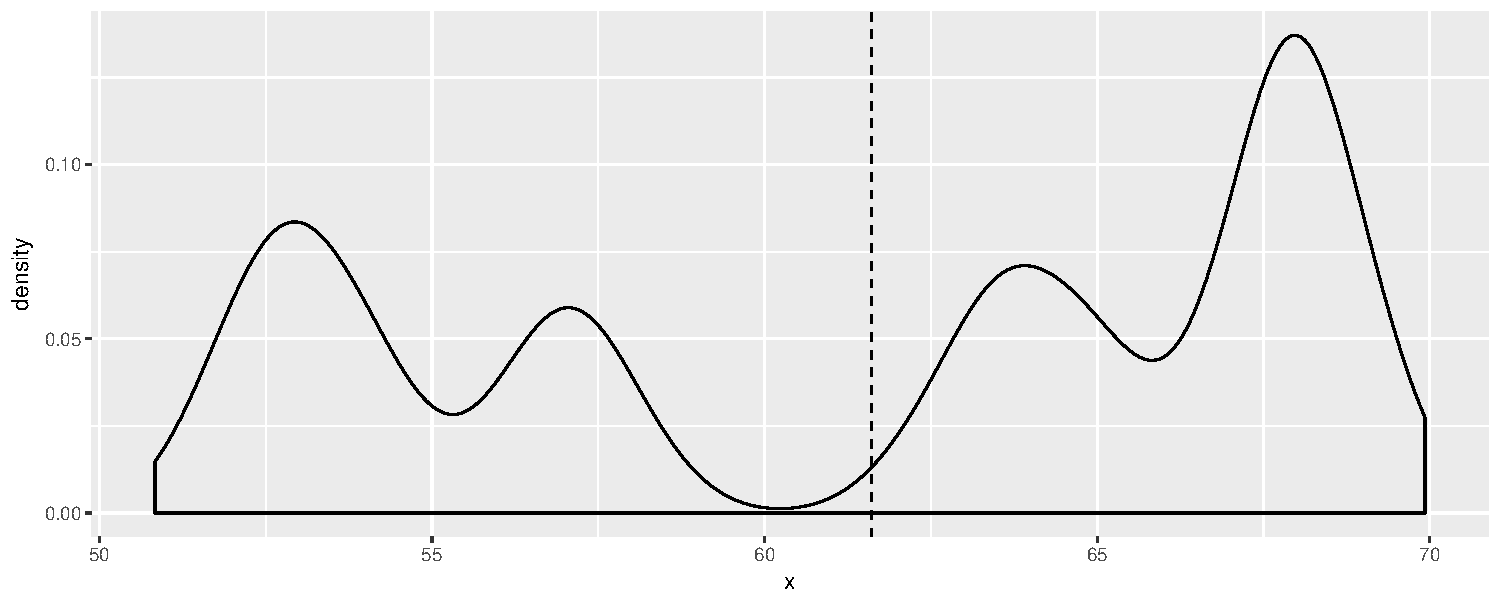
\includegraphics[width=\maxwidth]{figure/unnamed-chunk-2-1} 
\begin{kframe}\begin{alltt}
\hlkwd{coef}\hlstd{(}\hlkwd{lm}\hlstd{(wgt} \hlopt{~} \hlstd{hgt,} \hlkwc{data} \hlstd{= bdims))}
\end{alltt}
\begin{verbatim}
## (Intercept)         hgt 
## -105.011254    1.017617
\end{verbatim}
\end{kframe}
\end{knitrout}
 
\begin{enumerate}
  \itemsep0.7in
\item Describe the relationship between height and weight.
\item Write the equation of the regression line. Interpret the slope and intercept in context.
\item The correlation coefficient for height and weight is 0.72. Calculate $R^2$ and interpret it in context.
  \vspace{0.5in}
\end{enumerate}


\clearpage
\paragraph{One Categorical Explanatory Variable}

Recall our Rail Trail data example, and suppose that instead of using temperature as our explanatory variable for ridership on the RailTrail, we just used whether it was a weekday or not. The variable $weekday$ is \emph{binary} in that it only takes on the values 0 and 1. [Such variables are also called \emph{indicator} variables (by mathematicians) or \emph{dummy} variables (by economists).] Such a model has the form:
\begin{eqnarray*}
  \widehat{volume} = \hat{\beta}_0 + \hat{\beta}_1 \cdot weekday
\end{eqnarray*}

\begin{knitrout}\footnotesize
\definecolor{shadecolor}{rgb}{0.969, 0.969, 0.969}\color{fgcolor}\begin{kframe}
\begin{verbatim}
## (Intercept)    weekday1 
##   430.71429   -80.29493
\end{verbatim}
\end{kframe}
\end{knitrout}

\begin{enumerate}
  \itemsep0.5in
  \item How many riders does the model expect will visit the Rail Trail on a weekday? 
  \item How many riders does the model expect on a weekend? 
  \item What if it's a weekend and it's 80 degrees out?
  \item Draw a scatterplot of the data and indicate this model graphically.
  \vspace{1in}
  \item \emph{Estimate} the $R^2$ for this model. Is it greater or less than the $R^2$ for the model with temperature as an explanatory variable?
\end{enumerate}


\clearpage
\paragraph{Outliers, Leverage, and Influence}
It is important to identify the outliers and understand their role in determing the regression line.
\vspace{5in}
\begin{itemize}
  \itemsep0in
  \item An \emph{outlier} is an observation that doesn't seem to fit the general pattern of the data
  \item An observation with an extreme value of the explanatory variable is a point of high \emph{leverage}
  \item A high leverage point that exerts disproportionate influence on the slope of the regression line is an \emph{influential point}
\end{itemize}



\paragraph{Quick True or False}

  \begin{enumerate}
\item Influential points always change the intercept of the regression line.
\item Influential points always reduce $R^2$.
\item It is much more likely for a low leverage point to be influential, than a high leverage point.
  \end{enumerate}



% \newpage
% 
% \paragraph{Instructor's Notes}
% notes
% <<include=FALSE>>=
% require(mosaic)
% x = rnorm(100)
% y = rnorm(100)
% ds = data.frame(y,x)
% xyplot(y ~ x, data=ds, type=c("p", "r"), lwd=3)
% rsquared(lm(y ~ x, data=ds))
% @
% 
% 
% <<include=FALSE>>=
% ds = rbind(ds, data.frame(y=2, x=10))
% xyplot(y ~ x, data=ds, type=c("p", "r"), lwd=3)
% rsquared(lm(y ~ x, data=ds))
% @
% notes



\end{document}
